\documentclass[11pt,letterpaper]{article}
\usepackage{fullpage}
\usepackage{multicol}
\usepackage{amsmath}
\usepackage{amsfonts}
\usepackage{amssymb}
\usepackage{graphicx}
\usepackage{pstricks, pst-node, pst-plot}

\newcommand{\ds}{\displaystyle}
\newcommand{\bv}{\mathbf}
\newcommand{\lv}{\langle}
\newcommand{\rv}{\rangle}

\begin{document}
\flushleft
\begin{multicols}{2}


\begin{large}\textbf{Math 115 Quiz 10: $\oint $ 5.1-3 Summing Rectangles \\
Wed 8 December 2010}\end{large}

\textbf{Name:  }\underline{\hspace{35ex}}

\vspace{.5in}

\end{multicols}

\pagestyle{empty}

\flushleft

You have 30 minutes to complete this quiz.  Make your variables clear and
consistent (so if you want to say, for example, $\frac{dy}{dx}$, you should also
mention $y=f(x)$, or ``$y$ is a function of $x$'').  Calculators are OK.  

\begin{enumerate}
\item \textbf{Definitions/Concepts.} (1 pt each) True or False?  No explanation necessary.
\begin{enumerate}
 \item For an increasing function, the left-hand sum on a given interval with a given number of subdivisions is always less than the right-hand sum.

\vspace{0.5pc}
TRUE

\vspace{0.5pc}
\item A 4-term left-hand Riemann sum approximation cannot give the exact value of a definite integral.

\vspace{0.5pc}
FALSE

\vspace{0.5pc}
\item The units for an integral of a function $f(x)$ are the same as the units for $f(x)$.

\vspace{0.5pc}
FALSE
\end{enumerate}

\vspace{1.5pc}
\item \textbf{Questions/Problems.}  
\noindent Below you will write expressions for
each of various quantities indicated on the graph of
$f(x)$. Your
expressions may involve integrals or derivatives. For
example, if
asked for the ``$x$-coordinate of the point $P$,'' you
would write
``$a$''.

\begin{center}
 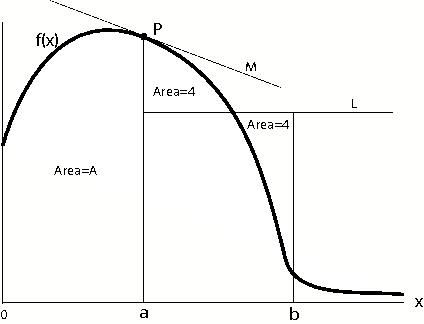
\includegraphics[scale=.8]{./q10.jpeg}
\end{center}

\noindent {\bf a)} (1 pt) The height (above the x-axis) of the
point P.

\[f(a)\]

\vspace{1.0pc}
\noindent {\bf b)} (1 pt)  The slope of the line M.

\[f'(a)\]

\vspace{1.0pc}
\noindent {\bf c)} (1 pt)  The size of the area A.

\[\int_0^af(x)dx\]

\vspace{1.0pc}
\noindent {\bf d)} (1 pt)  The height of the line L.

\[\frac{4}{b-a}\]   

\vspace{.05pc}
\emph{OR (for extra credit)} 

\[\frac{\int\limits_a^bf(x)dx}{b-a}\]

\vspace{0.5pc}
\item \textbf{Computations/Algebra.}  
\begin{enumerate}
\item  (1 pt) If $F(t)=\frac{1}{2}\sin{t^2}$, find $F'(t)$.

\[F'(t)=t\cos{t^2}\]

\vspace{0.5pc}
\emph{OR (this problem was a typo -- I meant to put $F(t)=\frac{1}{2}\left(\sin{t}\right)^2$)} 

\[F'(t)=\sin{t}\cos{t}\]

\vspace{1pc}
\item Find $\int_{0.2}^{0.4}\sin{t}\cos{t}dt$ two ways: 

\vspace{.5pc}
(i)  (1 pt) Numerically.  \emph{Use $n=4$ subdivisions then average the left and right -hand sums.  Tip for showing your work:  Use $\Sigma $-notation.}

\vspace{1pc}
In this case $\Delta t=0.05$ so the average will be

\begin{eqnarray*}
& \frac{1}{2}\left[0.05\left(\sin{0.2}\cos{0.2}+\sin{0.25}\cos{0.25}+\sin{0.3}\cos{0.3}+\sin{0.35}\cos{0.35}\right)+\right. \\
& \left.0.05\left(\sin{0.25}\cos{0.25}+\sin{0.3}\cos{0.3}+\sin{0.35}\cos{0.35}+\sin{0.2}\cos{0.2}\right)\right] \\
& \approx 0.0560
\end{eqnarray*}


\vspace{1pc}
(ii)  (1 pt) Using the Fundamental Theorem of Calculus.

\[\frac{1}{2}\sin{0.4^2}-\frac{1}{2}\sin{0.2^2}\approx 0.0597\]
\emph{OR, if you noticed the typo,}
\[\frac{1}{2}\left(\sin{0.4}\right)^2-\frac{1}{2}\left(\sin{0.2}\right)^2 \approx 0.0561\] 

\end{enumerate}

\end{enumerate}


%----------------------------------------------------------------------------------------

%\vspace{1pc}
%\noindent \textbf{ChAlLeNgE PrObLeM:}  
\end{document}


